% Partie fid : quelle mesure mène, et pourquoi un FID CNN à côté du FID Inception.
% Sources : PLAN.md §2, §5.1 ; enquete/fid.md ; baseline.md §3 ; enquete/results/juliet/{sensitivity_10k,kid_perclass_all}.csv ;
% enquete/results/fid/{rank_correlation,variance_share}.csv ; results/comparison_local.csv (sd entre seeds, ddof = 1).
% Plancher par chiffre : 8,5 (kid_perclass_all.csv 8,547) ; PLAN.md écrit 8,6 par erreur d'arrondi.
% Figure : figscripts/fid.py.
\section{Which FID? Evaluation}\label{sec:fid}

We add FID$_\text{CNN}$: in-domain (a LeNet replaces Inception on MNIST in~\cite{binkowski2018}), seconds instead of ${\approx}40$\,min of CPU (so tracked every epoch), and meant to see missing digits, the typical failure of an unconditional GAN.
The two FIDs can rank models oppositely: which should lead?

\paragraph{Measures.}
For features $\phi$ of real ($r$) and generated ($g$) images, with means $\mu$ and covariances $\Sigma$~\cite{heusel2017},
\[
\mathrm{FID}=\lVert\mu_r-\mu_g\rVert^2+\mathrm{Tr}\bigl(\Sigma_r+\Sigma_g-2(\Sigma_r\Sigma_g)^{1/2}\bigr).
\]
\textbf{FID$_\text{Inc}$}: $\phi$ = 2048-d pool layer of Inception-v3 (ImageNet).
\textbf{FID$_\text{CNN}$}: $\phi$ = 128-d penultimate layer of our MNIST classifier (98.7\% test accuracy).
\textbf{KID}: unbiased squared MMD, Inception features~\cite{binkowski2018}.
\textbf{P}: share of generated images inside the $k$-NN radius ($k{=}5$) of a real image, VGG features; \textbf{R}: real and generated swapped~\cite{kynkaanniemi2019}.
\textbf{Floor} (finite-$N$ bias~\cite{chong2020}): MNIST train vs test, 1.53 (Inc), 2.74 (CNN).

\paragraph{Expected.}
A FID follows the classes of its network~\cite{kynkaanniemi2023}: ImageNet has no digit class, our CNN has ten, so FID$_\text{CNN}$ should see the digit mix, FID$_\text{Inc}$ the appearance~\cite{heusel2017}.
Yet Lucic et al.\ find FID$_\text{Inc}$ on MNIST ``heavily influenced by the missing modes''~\cite{lucic2018}.

\begin{figure}[t]
\centering
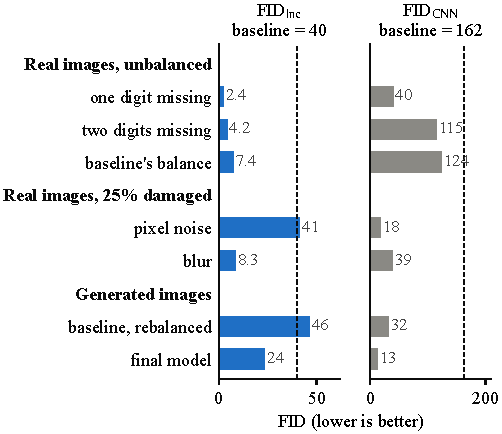
\includegraphics[width=\columnwidth]{fid_sensitivity}
\caption{\textbf{How much each FID sees each defect.} Each defect is added to real images; bar = its FID as a share of the baseline's gap to real data, $(\mathrm{FID}-\text{floor})/(\mathrm{FID}_\text{base}-\text{floor})$. $\mathrm{FID}_\text{base}$: baseline seed~0 (39.9 Inc, 162 CNN). Digit mix: 3 draws; other rows: one.}
\label{fig:fid-sensitivity}
\end{figure}

\paragraph{Observed.}
\begin{itemize}
\item \textbf{Dosed defects} (Fig.~\ref{fig:fid-sensitivity}): FID$_\text{Inc}$ weighs the digit mix about ten times less than FID$_\text{CNN}$, pixel noise ten times more; blur, blends and erasing weigh alike. Digit identity explains 67\% of the CNN feature variance, 26\% of Inception's.
\item \textbf{Rebalancing} baseline samples to the test digit mix: FID$_\text{CNN}$ 162\,$\to$\,32, but FID$_\text{Inc}$ \emph{rises} 39.9\,$\to$\,46.2 (badly drawn rare digits enter).
\item \textbf{Checkpoint:} FID$_\text{CNN}$ picks epoch 106, FID$_\text{Inc}$ epoch 200 ($\rho{=}{-}0.885$ after epoch 100): the digit imbalance grows while FID$_\text{Inc}$ falls.
\item \textbf{Seeds:} relative sd 11--25\% (FID$_\text{CNN}$) vs 3--6\% (FID$_\text{Inc}$), from the mix, not estimator noise (floor sd 0.19).
\item \textbf{KID} agrees with FID$_\text{Inc}$ (Spearman 0.96) and, like it, does not separate the baseline from raw RpGAN + R1 ($p=0.16$).
\end{itemize}

\paragraph{Per-digit FID$_\text{Inc}$.}
The CNN labels 100\,000 samples; 1\,000 per digit are scored against the test images of that digit; we average the ten (floor 8.5).
No frequency weighting: the baseline's ``2'' scores 113 (real 10.2) but makes up 1.6\% of images, so the global FID barely sees it (Sec.~\ref{sec:training}).
Limit: the CNN forces every image into a digit (confidence ${<}\,0.9$: 12.6\% of baseline images, 3.7\% of real ones).

\paragraph{When each measure fails.}
\begin{itemize}
\item \textbf{FID$_\text{CNN}$:} circular for instance selection (same features, Sec.~\ref{sec:data}); classifier-dependent (142--224 on the same images, three CNN seeds); saturating (final model: 6\% of the baseline gap vs 57\% in FID$_\text{Inc}$; on 6 RpGAN generators the FIDs disagree, $\rho{=}0.14$); it chose our $\gamma$ (Sec.~\ref{sec:training}); not comparable to papers or the platform.
\item \textbf{FID$_\text{Inc}$, P/R:} agree weakly with humans; DINOv2 is recommended~\cite{stein2023} (untested; we inspect samples, as the platform does).
\end{itemize}

\begin{table}[t]
\centering\footnotesize
\caption{\textbf{Which measure answers which question.}}
\label{tab:fid-roles}
\begin{tabular}{@{}ll@{}}
\toprule
Question & Measure \\
\midrule
Rank models, final scores & FID$_\text{Inc}$ + P/R (VGG, $k{=}5$) \\
Stroke quality at fixed digit & mean per-digit FID$_\text{Inc}$ \\
Digit mix & digit histogram (FID$_\text{CNN}$ as diagnostic) \\
Comparison with papers & FID$_\text{Inc}$ only \\
\bottomrule
\end{tabular}
\end{table}

\takeaway{FID$_\text{CNN}$ mostly measures the digit mix, FID$_\text{Inc}$ the appearance, and FID$_\text{Inc}$ even rewards dropping hard digits: use each measure for its own question (Table~\ref{tab:fid-roles}).}
